\documentclass{beamer}

\usecolortheme{UD}
 
\usepackage{tikz}
\usetikzlibrary{tikzmark}
\usetikzlibrary{arrows,shapes,backgrounds}
\usepackage{amsmath, amsfonts}

%\usepackage{enumitem}
\usepackage[UKenglish]{babel}
\usepackage{booktabs}
\usepackage{graphicx}
\usepackage{subfig}

\newcommand\DrawBox[6]{% 
	\begin{tikzpicture}[remember picture,overlay]
	\draw[red, ultra thick]([yshift=#3,xshift=#4]pic cs:#1) rectangle ([yshift=#5,xshift=#6]pic cs:#2);
\end{tikzpicture}%
}

\tikzstyle{every picture}+=[remember picture]
\tikzstyle{na} = [baseline=-.5ex]

\setbeamertemplate{itemize items}[circle]

\institute{
\includegraphics[height=1cm]{ud_logo}}

% -----------------------------------------------------------------------------
\graphicspath{ {figs/} }

%Information to be included in the title page:
\title{\bf{Background on Deep Learning}}
\author{Nate Merrill}
\subtitle{University of Delaware}

\begin{document}
 
\frame{\titlepage}


\begin{frame}{Popular Deep Learning Tasks}
        \begin{itemize}
            \item Classification
            \item Classifcation + Bounding Box Detection
            \item Muti-object detection
            \item Pixel-wise semantic segmentation
        \end{itemize}
        \begin{figure}
            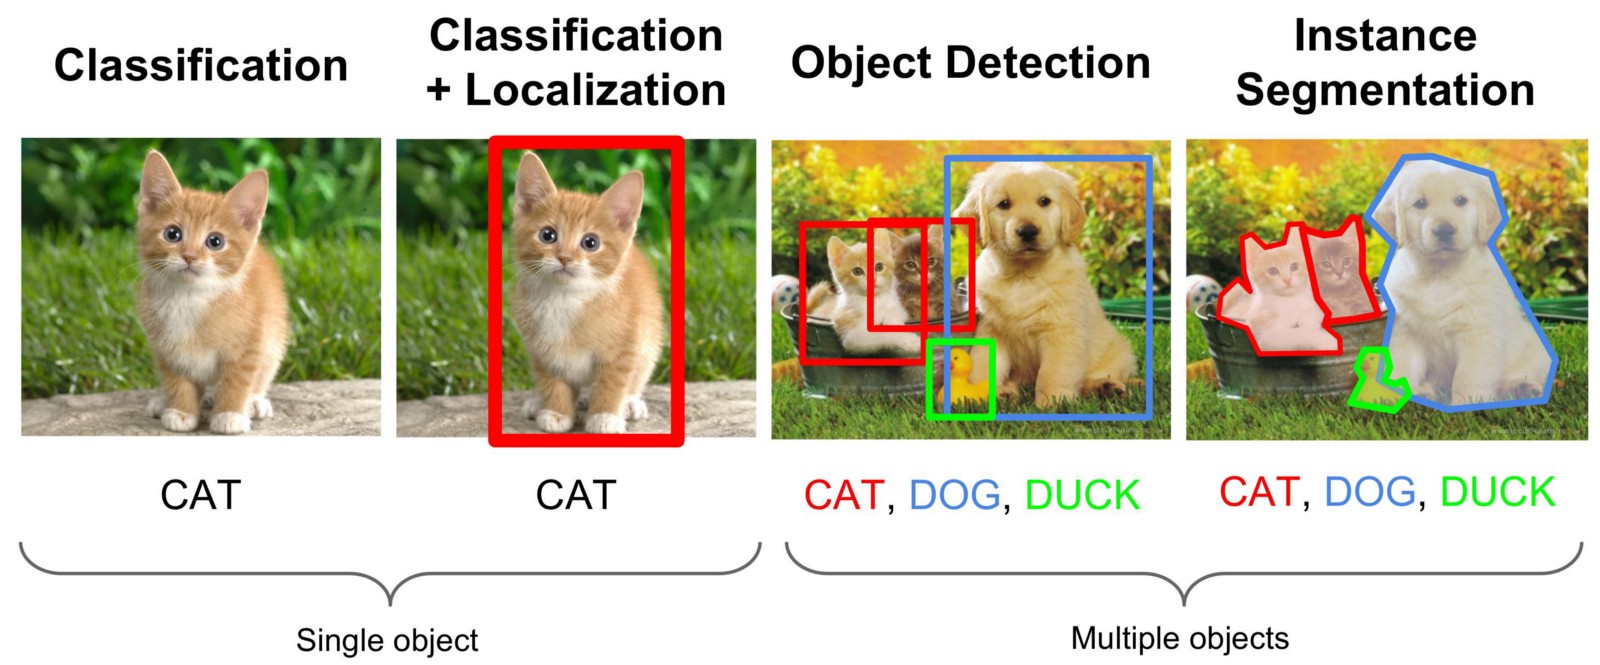
\includegraphics[width=\columnwidth]{kitties}
        \end{figure}
\end{frame}

\begin{frame}{More Popular Deep Learning Tasks}
        \begin{itemize}
            \item Embeddings (dimension reduction)
            \begin{itemize}
                \item Autoencoder
                \item Triplet Embedding
            \end{itemize}
        \end{itemize}
        
        \begin{columns}
            \column{.5\textwidth}
                \begin{figure}
                    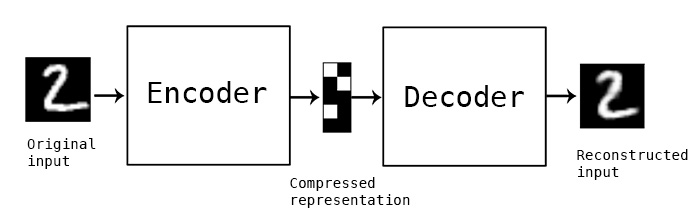
\includegraphics[width=\columnwidth]{autoencoder}
                    \caption*{Autoencoder}
                \end{figure}
            \column{.5\textwidth}
                \begin{figure}
                    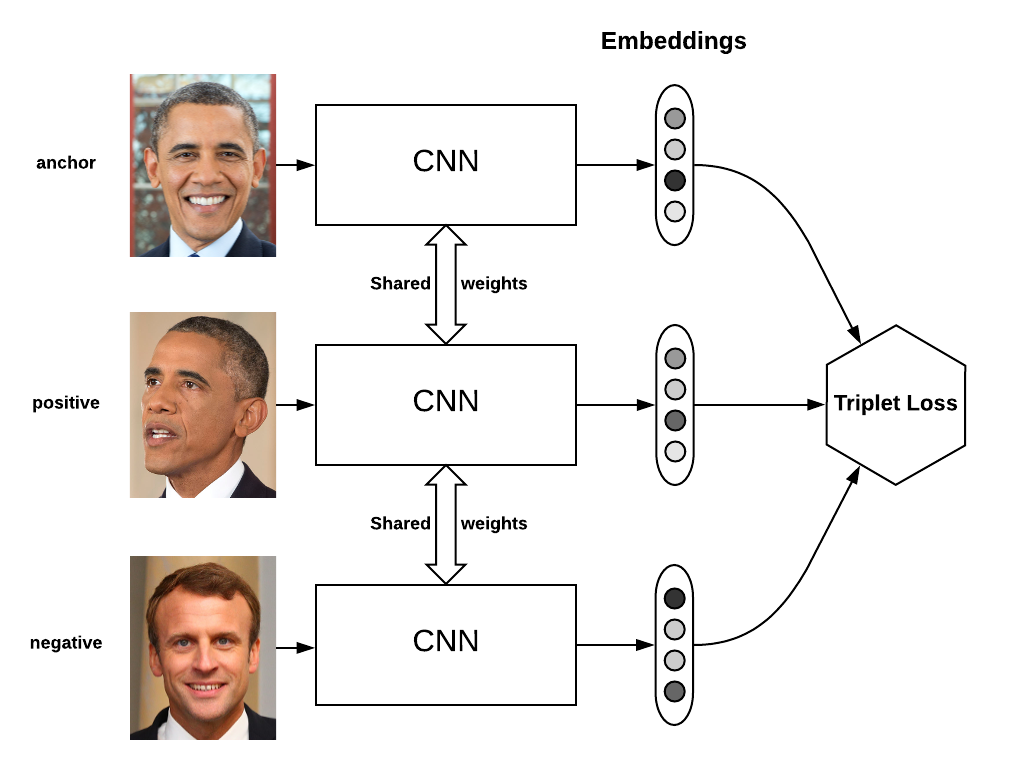
\includegraphics[width=\columnwidth]{triplet_embedding}
                    \caption*{Triplet embedding}
                \end{figure}
        \end{columns}
\end{frame}

\begin{frame}{Fully Connected Layer}
        \begin{columns}
            \column{.5\textwidth}
                \begin{itemize}
                    \item Vector input and output
                    \item Learned weights associated with each connection
                    \item Can be written as a linear operation  
                \end{itemize}
                \vspace{-10pt}
                \begin{align*}
                    \mathbf{x} &= \begin{bmatrix}x_1 & x_2 & \hdots & x_n & 1 \end{bmatrix}^\intercal \\
                     \mathbf{y} &= \begin{bmatrix}y_1 & y_2 & \hdots & y_m \end{bmatrix}^\intercal\\
                     \mathbf{W} &= \begin{bmatrix} w_{11} & w_{12} & \hdots & w_{1n} & b_1 \\
                                                 w_{21} & w_{22} & \hdots & w_{2n} & b_2 \\
                                                 \vdots & \ddots & \ddots & \vdots & \vdots \\
                                                 w_{m1} & w_{m2} & \hdots & w_{mn} & b_m \end{bmatrix} \\ 
                     \mathbf{y} &= \mathbf{W}\mathbf{x}
                \end{align*}

            \column{.5\textwidth}
                \begin{figure}
                    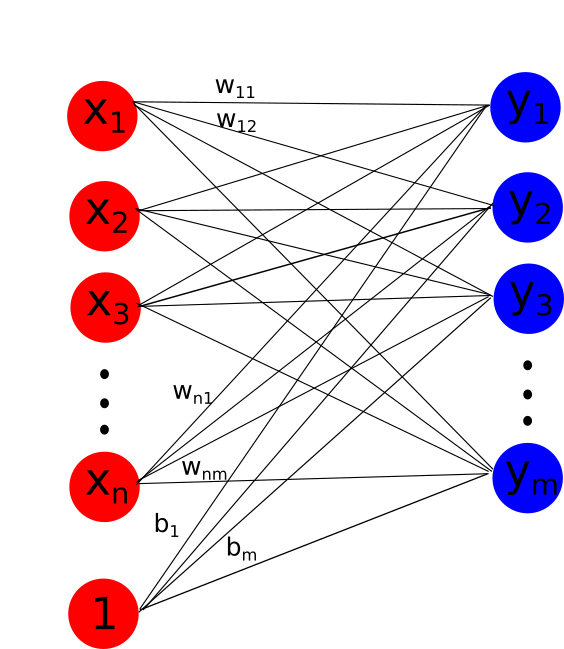
\includegraphics[width=\columnwidth]{fc}
                \end{figure}
        \end{columns}
\end{frame}

\begin{frame}{Nonlinear Activation}
    \begin{itemize}
        \item Fully connected layer cannot model nonlinear functions
        \item Nonlinear activations are used to provide nonlinearity
    \end{itemize}
    Examples:   
    \begin{figure}
        \hspace*{-2cm}
        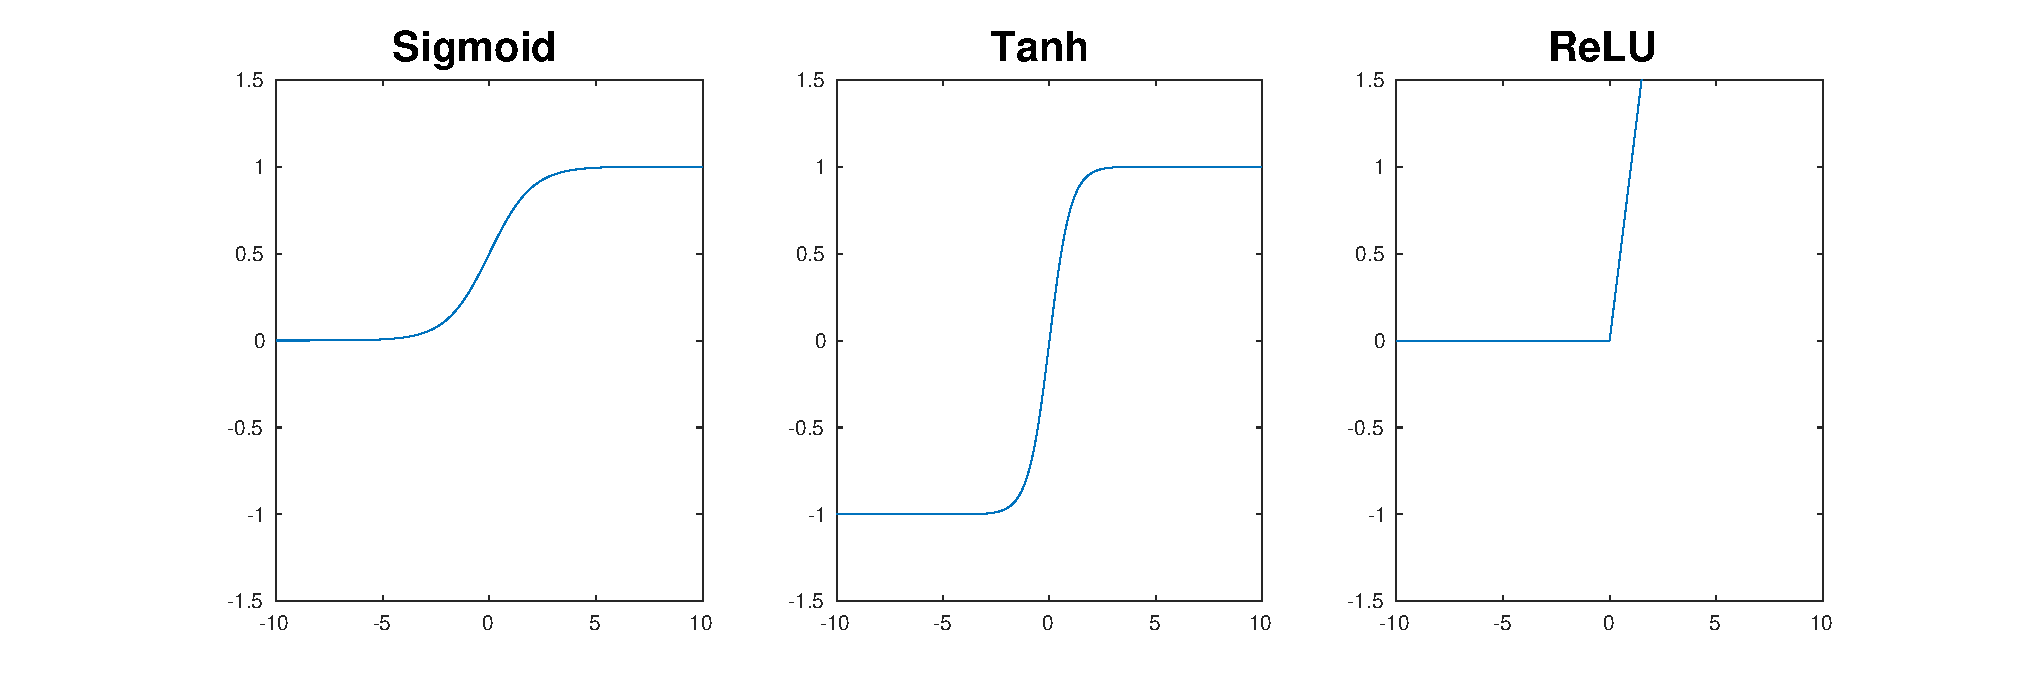
\includegraphics[width=1.33\textwidth]{activations}
        \caption*{Popular activation functions}
    \end{figure}

\end{frame}

\begin{frame}{Convolution Layer}
    \begin{itemize}
        \item Matrix/Tensor input and output
        \item Useful for image input
    \end{itemize}

    \begin{figure}
        \includegraphics[width=\textwidth]{conv}
    \end{figure}

    \vspace{-10pt}
    \begin{align*}
        Y_{ij} &= K_{33}X_{i,j} + K_{32}X_{i,j+1} + K_{31}X_{i,j+2} + K_{23}X_{i+1,j} \\
               &  + K_{22}X_{i+1,j+1} + K_{21}X_{i+1,j+2} + K_{13}X_{i+2,j} \\
               & + K_{12}X_{i+2,j+1} + K_{11}X_{i+2,j+2}
    \end{align*}
\end{frame}

\begin{frame}{Max Pooling Layer}
    \begin{itemize}
        \item Useful for viewpoint invariance
        \item Similar operation to convolution
    \end{itemize}


    \begin{figure}
        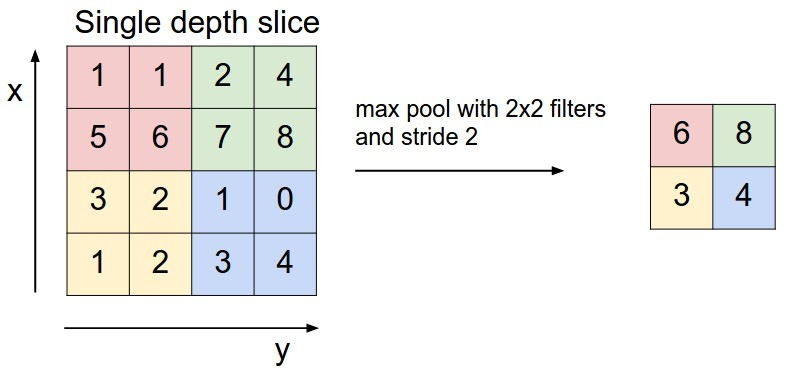
\includegraphics[width=\textwidth]{maxpool}
    \end{figure}
\end{frame}
\end{document}
